%
% chapter.tex -- Kapitel 3: 1-Formen und Kurvenintegrale
%
% (c) 2024 Prof Dr Andreas Müller
%
\chapter{Differentialformen und Kurvenintegrale
\label{chapter:kurvenintegral}}
\kopflinks{Differentialformen und Kurvenintegrale}
Ein Flug zum Mars muss Energie aufwenden, um gegen die Schwerkraft der
Sonne von der Erdbahn aus zu der 
Entfernung von der Sonne zu gewinnen.
In der Praxis wird dies dadurch erreicht, dass man dem Raumfahrzeug
mithilfe von Raketentriebwerken genügend kinetische Energie erteilt.
Es folgt dann einer elliptischen Bahn, die ihren sonnenfernsten Punkt
bei der Marsbahn hat.
Während des Fluges wird laufend kinetische Energie des Raumschiffs in
potenzielle Energie umgewandelt werden.
Mit jedem kleinen Teilstück der Flugbahn verliert das Raumschiff 
kinetische Energie, die proportional ist zur Kraftkomponente parallel
zur Flugbahn. 
Das potentielle Energiepaket das während des Teilstücks gewonnen wird,
ist linear vom Tangentialvektor der Bahn abhängig.
Die gesamte potentielle Energie, die zwischen Erde und Marsbahn
gewonnen wird, ist die Summe dieser Teilstücke.
Mathematisch wird es durch eine Art Integral einer Funktion dargestellt,
welches sowohl linear von der Bahntangente wie auch vom Pfad des
Raumschiffs abhängt.
Diese Integralkonstruktion muss aber so erfolgen, dass Sie nicht von der
Wahl von Koordinatensystemen und Parametrisierungen abhängt, was in
diesem Kapitel durchgeführt werden soll.
Sie muss ausserdem so funktionieren, dass sie sich über mehrer
Koordinatensysteme hinweg zusammensetzen lässt, wie dies bei einer
Bahn auf einer Mannifaltigkeit unvermeidlich wird.

%
% 1-Formen
%
\section{1-Formen}
Was ist es eigentlich, was man integrieren will?
Zunächst gibt der riemannsche Integralbegriff aus dem elementaren
Analysisunterricht den Eindruck, dass es eine Funktion ist.
Es können aber nicht allein die Funktionswerte sein, die das Integral
bestimmen.
Vielmehr kommt es auch darauf an, wie ``schnell'' der Definitionsbereich
beim Integrieren durchlaufen wird.
Dies wird zum Beispiel durch die Substitutionsformel für das Integral
wiedergegeben.
Man kann sie auch als eine Koordinatenänderungsformel für das Integral
entlang der reellen Achse betrachten.
Was ist dann aber die koordinatenunabhängige Grösse, deren Integral
bestimmt worden ist?
Dies soll in diesem Abschnitt geklärt werden.

%
% Riemann-Integral
%
\subsection{Riemann-Integral}
Im elementaren Analysis-Unterricht lernt man, dass das Riemann-Integral
\[
I
=
\int_a^b f(x)\,dx
\]
einer Funktion $f(x)$ die Fläche unter der Kurve $y=f(x)$ berechnet.
Man macht das, indem man die Fläche in zunächst in vertikale Streifen
der Breite $\Delta x_i$ zerlegt, die an bei den Koordinaten $x_i$
beginnen.
Die Rechtecke dürfen sich nicht überlappen und müssen die Fläche unter
der Kurve vollständig abdecken, die Teilstellen $x_i$ müssen
also $x_{i+1}=x_i+\Delta x_i$ erfüllen.
Dann ist die Summe
\begin{equation}
\sum_{i} f(x_i)\cdot \Delta x_i
\approx 
I
\label{buch:kurvenintegral:1-form:eqn:riemann-summe}
\end{equation}
eine Approximation für den Wert des Riemann-Integrals.

Der Unterschied zum exakten Wert kommt vor allem daher, dass die
Rechtecke mit Breite $\Delta x_i$ und Höhe $f(x_i)$ manchmal
die Funktionskurve überragen, zum Beispiel wenn die Kurve negative
Steigung hat, und manchmal darunter bleiben, wenn die Kurve positive
Steigung hat.
Der Unterschied setzt sich aus Dreiecken zusammen, deren Grundseite
$\Delta x_i$ ist, und deren Höhe durch $f'(x_i)\cdot \Delta x_i$
beschränkt ist.
Der Fehler ist daher grössenordnungsmässig nicht grösser als
\[
\Delta I
\approx
\sum_i \Delta x_i \cdot |f'(x_i)\cdot \Delta x_i|
=
\sum_i |f'(x_i)| \Delta x_i^2.
\]
Sorgt man dafür, dass die Schritte $\Delta x_i$ alle gleich klein
sind, also $\Delta x_i=h$, dann folgt
\[
\Delta I
\approx
\sum_i |f'(x_i)| h^2
=
h\sum_i |f'(x_i)|h
\approx
h\int_a^b |f'(x)|\,dx.
\]
Für eine stetig differenzierbare Funktion ist $f'(x)$ im Integranden
auf der rechten Seite beschränkt.
Das Integral auf der rechten Seite ist also beschränkt.
Es bleibt aber der Faktor $h$, der den Fehler $\Delta I$ beliebig
klein macht, wenn man $h$ gegen $0$ gehen lässt.

%
% Substitution
%
\subsection{Substitution}
Der Integrand $f(x)$ im Riemann-Integral ist offenbar eine von
der Parametrisierung unabhängige Grösse.
Wechselt man die Koordinaten mit Hilfe einer Koordinatentransformation
$x(y)$, dann bleiben die Werte $f(x(y))$ an entsprechenden Stellen
des Definitionsbereiches die gleichen.
Es ändert sich aber das durch den Faktor $dx$ im Integral symbolisierte
Gewicht, mit dem jeder Summand in der Riemann-Summe
\eqref{buch:kurvenintegral:1-form:eqn:riemann-summe}
gewichtet wird.
Die Koordinatentransformation $x(y)$ macht aus einem Schritt $\Delta y$
einen $x$-Schritt von der Grössenordnung
\[
\Delta x
\approx
\frac{dx}{dy}(y)\cdot \Delta y.
\]
Sind $a'$ und $b'$ die Endpunkte des $y$-Intervalls, die auf 
$a=x(a')$ und $b=x(b')$ abgebildet werden, dann ist daher das
Integral
\begin{equation}
\int_a^b f(x)\,dx
=
\int_{a'}^{b'} f(x(y)) \, \frac{dx}{dy}(y)\,dy.
\label{buch:kurvenintegral:1-form:eqn:substitution}
\end{equation}
Dies ist die bekannt Formel für die Substitutionsformel für das Integral.


%
% Integral über ein eindimensionales Definitionsgebiet
%
\subsection{Integral über ein eindimensionales Definitionsgebiet}
%
% fig-1koordinaten.tex
%
% (c) 2025 Prof Dr Andreas Müller
%
\begin{figure}
\centering
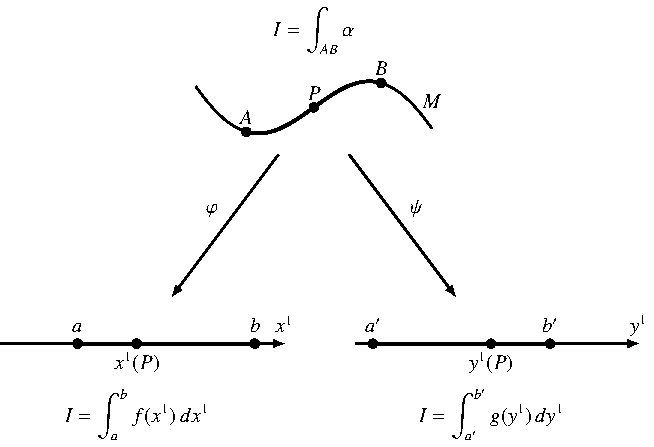
\includegraphics{chapters/030-kurvenintegral/images/1koordinaten.pdf}
\caption{Verschiedene Koordinatensysteme für ein eindimensionales
Definitionsgebiet $M$, auf dem ein Integral berechnet werden soll.
Oben steht ein koordinatensystemunabhängiges Konzept für eine Integral, 
welches in verschiedenen Koordinaten durch ein Riemannsches Integral
berechnet werden kann.
Die Substitutionsformel für das Integral liefert das
Koordinatentransformationsgesetzt zwischen den Darstellungen
$f(x^1)\,dx$ und $g(y^1)\,dy^1$ von $\alpha$.
\label{buch:kurvenintegral:fig:1koordinaten}}
\end{figure}

Die Substitutionsformel erklärt, wie das Integral angepasst werden
muss, wenn man von einer Koordinatenwahl $x$ zur alternativen
Koordinate $y$ wechseln will.
Wir können das Integral aber auch als eine Zahl betrachten,
die nur von zwei rein geometrisch definierten Eigenschaften
abhängig sind.
Einerseits ist dies eine Teilmenge eines eindimensionalen
Definitionsgebietes, welches in
Abbildung~\ref{buch:kurvenintegral:fig:1koordinaten} durch
den Bereich zwischen den Punkten $A$ und $B$ entlang der Menge $M$
symbolisiert ist.
Durch die Koordinatenssysteme $\varphi$ und $\psi$ werden daraus
die Intervalle $[a,b]$ von $x^1$-Koordinatenwerten bzw.~$[a',b']$
von $y^1$-Koordinatenwerten.

Die zweite Komponente zur Definition des Integrals ist eine
noch zu definierende Grösse $\alpha$, die die Funktionswerte
entlang des Definitionsgebietes liefert.
Dies muss so geschehen, dass $\alpha$ wieder ein Objekt ist,
welches vom Koordinatensystem unabhängig definiert ist, oder 
besser, dessen Transformationseigenschaften beim Koordinatenwechsel
klar sind.
Als Leitlinie für die gesuchte Umrechnungsformel kann die
Substitutionsformel
\eqref{buch:kurvenintegral:1-form:eqn:substitution}
herangezogen werden.

Das gesamte Integral möchten wir als
\[
\int_{AB} \alpha
\]
schreiben können.
Es soll die üblichen Eigenschaften eines Integrals haben, also
insbesondere linear sein:
\[
\int_{AB}
(\alpha + \beta)
=
\int_{AB}
\alpha
+
\int_{AB}
\beta
\qquad\text{und}\qquad
\int_{AB}
t
\alpha
=
t
\int_{AB}
\alpha.
\]
In einem Koordinatensystem soll eine Integralformel entstehen.
Rein formal ist daher $\alpha$ in den Koordinatensystemen $\varphi$
bzw.~$\psi$ durch
\[
f(x^1)\,dx^1
\qquad
\text{bzw.}
\qquad
g(y^1)\,dy^1
\]
gegeben.
Die Substitutionsformel
\eqref{buch:kurvenintegral:1-form:eqn:substitution}
besagt dann, dass
\[
g(y^1)
= 
f(\varphi\circ\psi^{-1}(y^1))
\frac{dx^1}{dy^1}(y^1)
=
f(\varphi\circ\psi^{-1}(y^1))
\frac{d}{dy^1}(\varphi\circ\psi^{-1}(y^1))
\]
sein muss.
Man beachte, dass $g(y^1)$ und $f(x^1)$ nicht Komponenten eines
Vektors sind, dann für Vektorkomponenten $v_1$ gilt wegen
\[
\frac{\partial}{\partial y^1}
=
\frac{dx^1}{\partial y^1}\cdot \frac{\partial }{\partial x^1}.
\]
die Umrechnungsformel
\[
v_1'(y^1)
=
\frac{dy^1}{dx^1}
v_1(x^1)
\qquad\text{oder}\qquad
v_1(x^1)
=
\frac{dx^1}{dy^1} v_1'(y^1).
\]
Die Transformation erfolgt also in der ``falschen'' Richtung.

Aus der Sicht des angestrebten Ziels, ein koordinatenunabhängiges
Integralkonzept zu definieren, ist die gegenüber Vektoren ``verkehrte''
Transformationsrichtung zu erwarten.
Wenn ein Koordinatenwechsel dazu führt, dass der Koordinatenraum
langsamer durchlaufen wird, äussert sich das darin, dass die Komponenten
eines Tangentialvektors grösser werden.
Der Tangentialvektor beschreibt aber die ``Schrittgrösse $dx$'' beim
Integrieren auf koordinatenunabhängige Art.
Damit das Integral gleich bleibt, muss der skalare Faktor entsprechend
kleiner werden.

%
% Transformation von Linearformen
%
\subsection{Linearformen}
Die im vorangegangenen Abschnitt heuristisch hergeleitete
Transformationseigenschaft ist nicht so überraschend, man kann sie
auch in der linearen Algebra bei Linearformen finden.
In diesem Abschnitt soll die Koordinatentransformationsregel für
Linearformen formuliert werden.

\subsubsection{Koeffizienten einer Linearform}
Seien $a^i$ die Komponenten eines Vektors $a$ in einer Basis $e_i$ und
$t_{i}\mathstrut ^k$ die Koeffizienten der Transformationsmatris
in eine alternative Basis $e'_k$.
Die Komponenten in der alternativen Basis werden mit $a^{\prime k}$
bezeichnet und die Umrechung zwischen den Koordinaten erfolgt mit der
Formel
\begin{equation}
a^{\prime k}
=
t_i\mathstrut^k a^i
\label{buch:kurvenintegral:1formen:linearformen:vektor}
\end{equation}
gegeben.

Eine Linearform ist eine lineare Abbildung $l\colon V\to\mathbb{R}$,
die einem Vektor $v$ einen Zahlenwert $l(v)$ zuordnet.
Die Linearität verlangt, dass der Wert
\[
l(a)
=
\sum_i
l(a^ie_i)
=
a^i \underbrace{l(e_i)}_{\displaystyle=l_i}
\]
ist (man beachte die einsteinsche Summationskonvention).
Die Werte $l_i=l(e_i)$ sind die Koeffizienten, mit denen die $a^i$
multipliziert werden müssen, um $l(a)$ zu ergeben.
Entsprechend sind die $l'_i=l(e'_i)$ die Koeffizienten der Basis

\subsubsection{Transformation der Koeffizienten einer Linearform}
Bei der Koordinatentransformation soll sich der Wert $l(a)$ nicht
ändern, es muss daher
\[
l'_k
a'^k
=
l'_k
(t_i\mathstrut^k a^i)
=
(l'_kt_i\mathstrut^k) a^i
=
l_i
a^i
\]
sein.
Da dies für jeden beliebigen Vektor gelten muss, müssen die Koeffizienten
übereinstimmen und es folgt das Transformationsgesetz
\begin{equation}
l'_kt_i\mathstrut^k
=
l_i
\label{buch:kurvenintegral:1formen:linearformen:linearform}
\end{equation}
für die Koeffizienten der Linearform.
Die Transformation der Linearformkoeffizienten erfolgt also
in der umgekehrten Richtung vom gestrichenen Koordinatensystem 
zum ungestrichenen.
Ausserdem wird über den obneren Index von summiert statt über
den unteren wie in 
\eqref{buch:kurvenintegral:1formen:linearformen:vektor}.

Betrachtet man die Koeffizienten $t_i\mathstrut^k$ als Matrix, mit der
die Umrechnung der Koeffizienten von $a$ erfolgt, dann ist die Matrix,
mit der die Koeffizienten $l_k'$ umberechnet werden, die transponierte
Matrix.

\subsubsection{Kovariante und kontravariante Indizes}

\subsubsection{Integrand $\alpha$ als Linearform}

%
% Die Koordinaten-1-Formen
%
\subsection{Die Koordinaten-1-Formen}

%
% Kurvenintegral einer 1-Form
%
\section{Kurvenintegral einer 1-Form}

%
% Differential einer Funktion
%
\section{Differential einer Funktion}

%
% Differenzierbare Zerlegungen der Einheit
%
\section{Differenzierbare Zerlegung der Einheit}
Ein Wegintegral kann sich entlang eines Pfades erstrecken, der
mehrere Kartengebiete einer Mannigfaltigkeit durchauert.
Das Kurvenintegral ist mithilfe eines Koordinatensystems definiert,
kann also immer nur innerhalb eines Kartengebietes berechnet werden.
Es muss also ein Technik gefunden werden, mit der Teilintegrale in
einzelnen Kartengebieten zu einem Integral über die ganze Kurve
zusammengesetzt werden.
Die Konstruktion muss von der Wahl der Koordinatensysteme enthlange
des Pfades unabhängig sein.
Dies wird erreicht mit einer differenzierbaren Zerlegung der Einheit
und dank der Tatsache, dass das Kurvenintegral linear in der 1-Form
ist.

\subsection{Glatte Funktionen mit Träger in einem Interval}

\subsection{Überdeckung mit offenen Intervallen}

\subsection{Differenzierbare Zerlegung der Einheit}

\subsection{Zerlegung eines Kurvenintegrals}


